In today's rapidly evolving technological landscape, building robust, scalable,
and maintainable systems is paramount. A well-designed system architecture not
only addresses these needs but also provides a foundation for future growth and
adaptability. This section delves into the architecture that underpins our
system, exploring the principles of microservices, the application of Clean
Architecture, and the integration of various infrastructure components to create
a cohesive and efficient solution.

\subsection{Microservices}

In essence, a microservices architecture decomposes a large software application
into a collection of smaller, self-contained services. Each service plays a
specific role and owns a well-defined business capability. These services are
loosely coupled, meaning they interact through well-designed APIs and operate
independently.

Microservices architectures offer a compelling approach to building software. By
decomposing large applications into smaller, independent services, they unlock
agility, maintainability, and fault isolation.  Each service owns a specific
business function and interacts with others through well-defined APIs. This
allows for faster development cycles, easier maintenance of individual services,
and the freedom to choose the best technology for each job.

However, this power comes with a price. Managing a distributed system with
numerous services inherently increases complexity compared to a monolithic
application. Communication between services adds overhead to the system's
performance. Perhaps the most significant challenge lies in ensuring data
consistency across these independent services, requiring meticulous design and
implementation.  Carefully considering these trade-offs is crucial before
embarking on a microservices journey.

While microservices boast impressive agility and maintainability, adopting this
architecture isn't without its complexities.  Managing a distributed system with
numerous services inherently increases complexity compared to a monolithic
application.  Furthermore, communication between these services adds overhead to
the system's performance.  Perhaps the most significant challenge lies in
ensuring data consistency across these independent services, requiring
meticulous design and implementation.

\subsection{Clean Architecture}

Microservices and Clean Architecture can complement each other to create a
modular, maintainable, and scalable system. Microservices architecture promotes
the development of small, independent services that can be deployed, scaled, and
updated independently. Each microservice encapsulates a specific business
capability or domain, reducing the overall complexity of the system.

Clean Architecture, on the other hand, advocates for a layered approach to
software design, promoting separation of concerns and decoupling of components.
By adhering to the principles of Clean Architecture within each microservice,
developers can achieve a high degree of modularity, testability, and
maintainability.

Clean Architecture separates the system into distinct layers, each with specific
responsibilities. The Shared Kernel acts as the core, housing reusable
components that benefit all layers. The Domain layer sits at the heart of the
application, defining core entities and their behaviors. A common base class
promotes code maintainability within this layer. The Application layer
orchestrates request routing and establishes project-wide contracts for
implementation in other layers. Clean Architecture emphasizes the testability of
each layer through unit tests. Frameworks like xUnit simplify unit test
creation. 

The Infrastructure layer provides supporting services for the application.
Cross-cutting concerns like logging reside here. User registration,
authentication, and authorization functionalities are handled by the Identity
layer. Persistence takes care of data access using patterns like repositories
and Unit of Work. The Web Framework layer manages configurations for the web
application, while the Web API layer delivers functionality to the user.
Finally, plugins bridge the gap between monolithic and microservices
architectures by promoting modularity.

\subsection{Recommended System Architecture}

\begin{figure}[H]
    \centering
    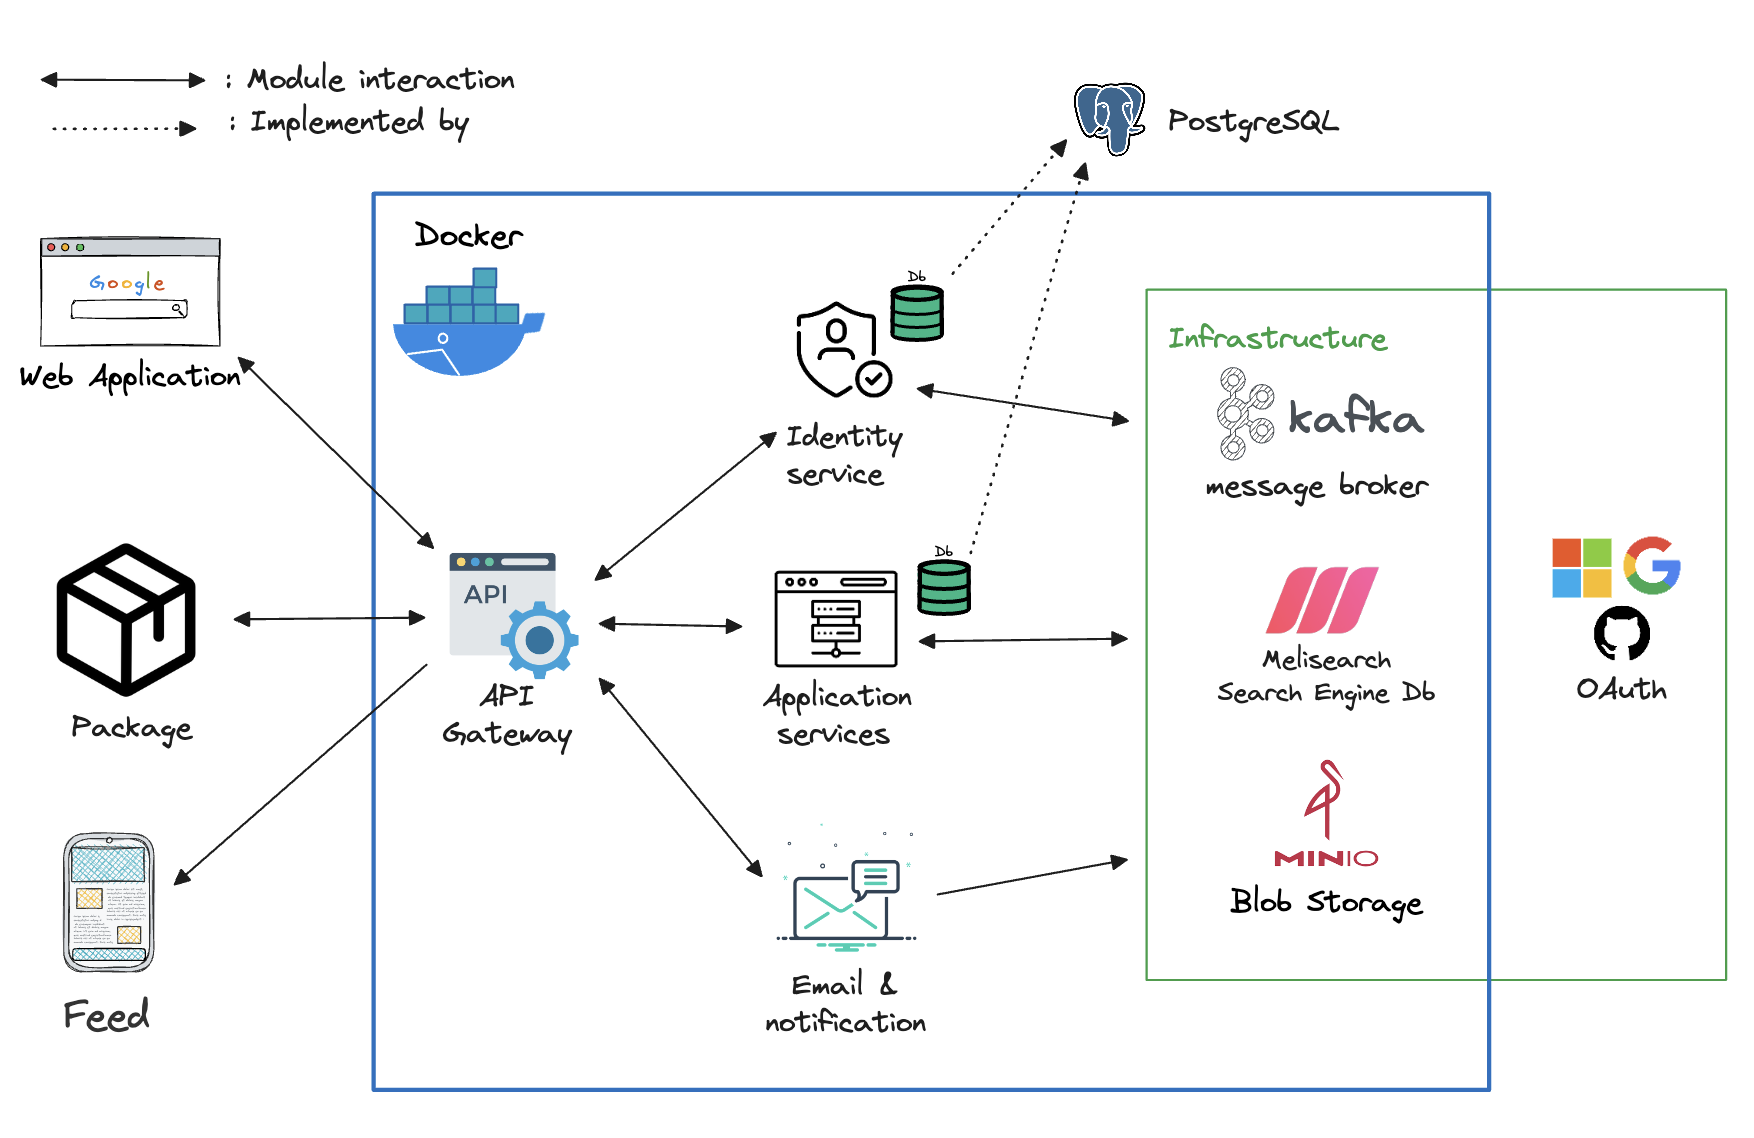
\includegraphics[width=\linewidth]{Images/arch.png}
    \vspace{1em}
    \caption{System Architecture}
    \label{fig:sow}
\end{figure}
\vspace{0.5cm}
Based on the requirements set by stakeholders and after studying the existing
system, the team proposes the design and implementation of a Weather Data
Platform. Figure \ref{fig:sow} illustrates the implementation of the system.

Central to this architecture is the use of Docker, which encapsulates the
application's microservices in containers. This encapsulation ensures that each
service can be deployed and scaled independently across different environments
without compatibility issues. Docker not only facilitates easy deployment but
also enhances the manageability and scalability of the application services,
making the infrastructure robust and flexible.

Within this architecture, a critical component is the Identity Service. This
service is responsible for managing user authentication and authorization
processes. It likely operates with a dedicated database that stores user
credentials and session information, ensuring secure and efficient user access
control. By centralizing identity management, the system can enhance security
and simplify the integration of different services that require user
identification and access control.

The Application Services form the backbone of the system's business logic. These
services handle the core functionalities of the application, interacting with
the Identity Service for authentication purposes and accessing dedicated
databases to retrieve or store data. This separation of concerns allows for
better maintenance and scalability of the application logic, enabling each
service to be optimized and scaled according to specific demands without
affecting the overall system performance.

An Email \& Notification Service is integral to the architecture, managing
communications with users. This service automates the sending of emails and
other notifications, which are crucial for user engagement and timely
communication. By having a dedicated service for this function, the system
ensures that notifications are handled efficiently, maintaining high performance
even under heavy loads of communication tasks.

The architecture is further supported by robust infrastructure components.
PostgreSQL serves as the primary database management system, offering reliable
and efficient management of structured data with its powerful SQL capabilities.
Kafka, used as a message broker, ensures seamless and reliable data flow between
different parts of the application, which is essential for maintaining data
consistency and decoupling services. Meilisearch enhances the application's
functionality by providing a fast and responsive search engine database, which
significantly improves the user experience through quick search results. MinIO
offers a high-performance solution for blob storage, managing unstructured data
such as media files, backups, and logs, which supports the application’s
scalability and data management needs. Lastly, OAuth is employed to facilitate
secure delegated access, allowing the application to authenticate users by
integrating with external OAuth providers like Google, thus broadening the scope
of user accessibility and security.

Each component of this architecture plays a vital role in ensuring the
application is scalable, modular, and resilient, employing a combination of
state-of-the-art tools and technologies to meet a broad range of operational
requirements efficiently.
